\chapter{Үр дүн}

Машин сургалтанд ашиглах өгөгдлийн тоо хэмжээ аль болох их байх нь сургалтын үр дүн, үзүүлэлтэнд сайнаар нөлөөлдөг. Энэхүү судалгааны ажлыг гүйцэтгэх хугацаанд эхлээд ерөнхий судалгаа хийж ямархуу байдлаар санг үүсгэх, боловсруулалт хийх, боловсруулалт хийх програмыг хөгжүүлэх, засах болон сайжруулах ажлуудыг гүйцэтгэн үлдсэн хугацаанд машин сургалтанд ашиглахад бэлэн болсон эсвэл тодорхой үр дүн харуулах хэмжээний өгөгдөл цуглуулж амжаагүй учир  одоогийн байдлаар ямар тэмдэгтүүд тус бүрт хэр их хэмжээний өгөгдөл/зураг цуглуулсан байгааг Зураг \ref{fig:result} -д харуулав.

\begin{figure}[ht]
	\centering
	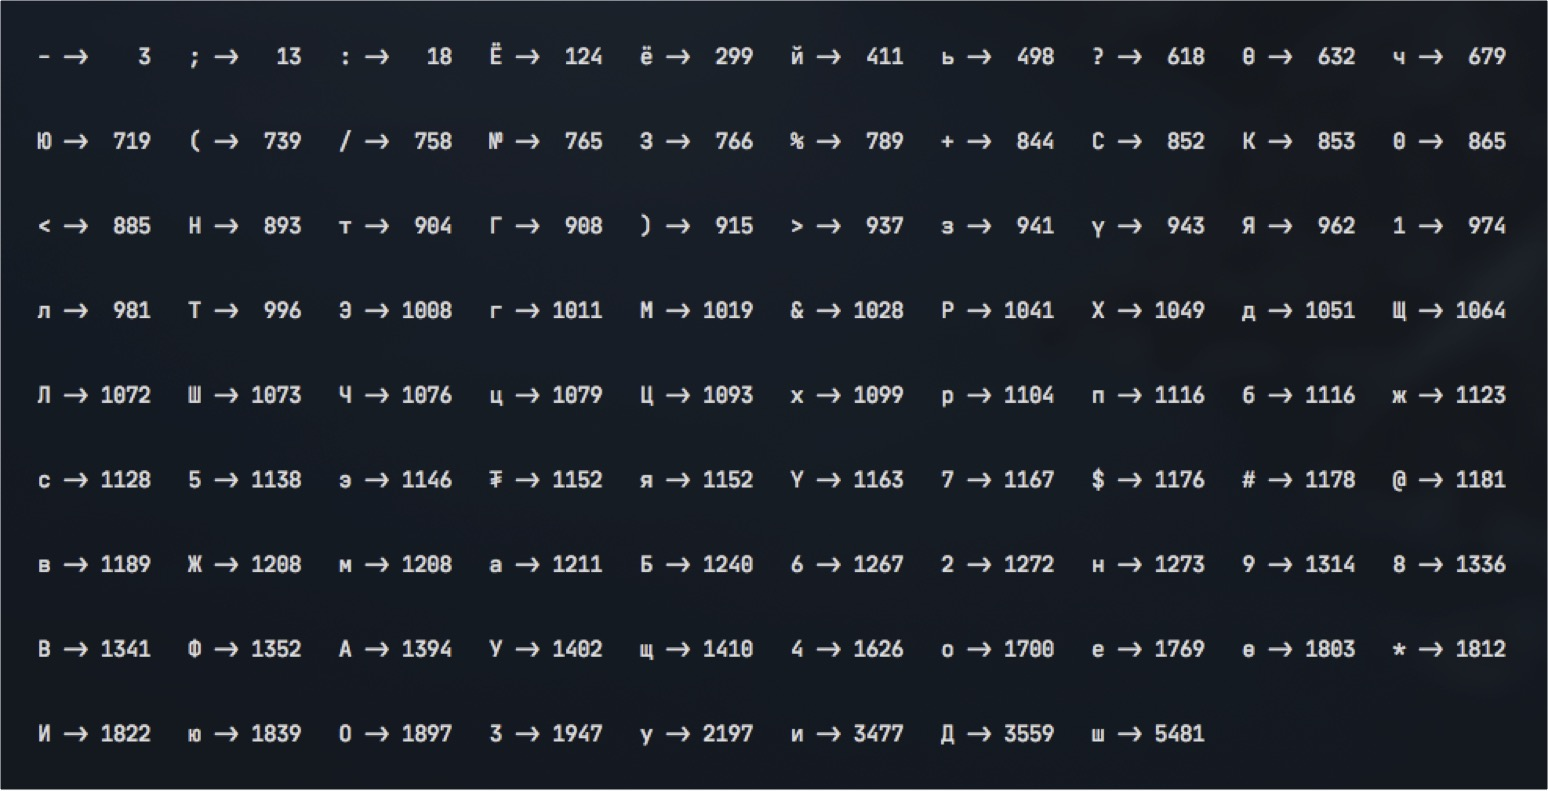
\includegraphics[width=1\linewidth]{images/result.jpg}
	\caption{Цугларсан тэмдэгт бүрт харгалзах өгөгдөл/зургийн тоо}
	\label{fig:result}
\end{figure}

Дээрх өгөгдлийн дийлэнхи хувь нь удирдагч багшийн \textit{“Гинжин кодын аргаар Монгол хэлний гар бичмэл танилт”} \cite{mongolian-htr-using-chain-code} судалгааны ажлын хүрээнд цуглуулан ялгасан тэмдэгтийн зургуудийг өөрийн боловсруулалтын аргаар боловсруулан үүсгэсэн өгөгдлөөс бүрдсэн ба цаашид оролтын маягтыг аль болох олон хүнээр бөглүүлэн өгөгдлийн хэмжээг ихэсгэх шаардлагатай.